% !TeX root = Stageportfolio.tex



\begin{landscape}
	Mijn stage werd vroegtijdig beëindigd vanwege de sluiting van de scholen omtrent de maatregelen die voltrokken werden vanwege Covid-19. Hieronder wil ik toch mijn reeds getroffen voorbereidingen plaatsen: de lesvoorbereiding (weliswaar met nog onvolledige beginsituatie en acties) van les 21 en het labo dat ik tijdens les 22 en 23 zou begeleiden.
	
	\subsubsection{Les 21}
	
	\begin{tabularx}{1.56\textwidth}{|p{0.35\textwidth}|X|}\hline
		\textbf{Administratieve gegevens}\newline\newline
		Kevin Truyaert\newline\newline
		technisch secundair onderwijs\newline
		3e graad, 1ste jaar, Techniek-Wetenschappen\newline
		VVKSO: \href{http://ond.vvkso-ict.com/leerplannen/doc/Toegepaste\%20fysica-2014-041.pdf}{http://ond.vvkso-ict.com/leerplannen /doc/Toegepaste\%20fysica-2014-041.pdf} \newline
		\underline{Lesonderwerp}:\newline De transformator en het elektrisch energietransport  & \textbf{Doelstellingen}
		\begin{itemize}[itemsep=0.08\baselineskip]
			\item B28: Met behulp van de wet van Lenz de zin van de inductiespanning vinden.
			\item B29: De algemene inductiewet hanteren.
			\item B31: De transformatorhouding bij de spanningen en de stromen van een ideale transformator toepassen en zijn functie bij het transport van elektrische energie toelichten.
		\end{itemize}
		\underline{Lesdoelen}\newline
		\vspace{-0.75cm}
		\begin{enumerate}[itemsep=0.08\baselineskip]
			\item De leerlingen kunnen het doel van een transformator verwoorden.
			\item De leerlingen kunnen de zin van de inductiestroom bepalen.
			\item De leerlingen kunnen de wet van Faraday-Lenz hanteren.
			\item De leerlingen kennen de transformatieverhouding voor spanningen bij een transformator.
			\item De leerlingen kennen de transformatieverhouding voor stromen bij een transformator.
			\item De leerlingen begrijpen de werking van een transformator.
			\item De leerlingen begrijpen waarom elektrische energie bij hoge spanningen vervoerd wordt. 
			\item De leerlingen kunnen het afgelegde traject tussen centrale en het stopcontact schetsen.
			\item De leerlingen kunnen de transformatieverhouding voor spanningen in oefeningen toepassen.  
			\item De leerlingen kunnen de transformatieverhouding voor stromen in oefeningen toepassen.  
		\end{enumerate} \\\hline
	\end{tabularx}\vfill \textcolor{white}{.} 


	\begin{tabularx}{1.56\textwidth}{|p{0.55\textwidth}|X|}
		\hline
		\multirow{2}{0.55\textwidth}{\textbf{Beginsituatie}\newline  
		Er zijn acht leerlingen binnen 5TW. Er heerst een algemene klassfeer. De leerlingen hebben al theorie gekregen  rond en oefeningen gemaakt op de magnetische krachtwerking. \newline\newline De leerlingen hebben vorige week de wisselspanningsgenerator gezien als een toepassing van magnetische inductie. Daarnaast kregen ze ook al een inleiding tot de transformator \newline\newline NOG AANVULLEN MET LERAARKENMERKEN.} & \textbf{Acties}\newline\newline 
		- \YellowHighlight{De transformator is een stuk fysica die in ons dagelijkse leven onbewust vaak}{15cm} \YellowHighlight{gebruikt wordt.}{3cm} Het zit in alle adapters die we gebruiken. Daarom is het belangrijk dat dit ook in de fysicales besproken wordt om de werking ervan te begrijpen.	 \newline\newline 
		\newline\newline\newline\newline\newline\newline
		
		\\ \cline{2-2}
		  & \textbf{Bronnen}\begin{itemize}
		  	\item Schramme, S. (2018) De stroombalans, labo magnetisme 4
		  	\item Frederiksen (2014), Current Balance 4565.00
		  	\item Giancoli, D. C. (2008). Physics for scientists and engineers. Pearson Education International.
		  \end{itemize}\\ \hline
	\end{tabularx}


\newpage
	
	\begin{tabularx}{1.56\textwidth}{|p{1.5cm}|p{8cm}|X|p{4cm}|}
		\hline
		\textbf{Nr. lesdoel } & \textbf{Inhoud (timing)}  & \textbf{Organisatie } & \textbf{Media } \\ \hline
		1&\underline{Herhaling wat is transformator (5 minuten)}\newline
			De leerlingen herhalen de componenten en het doel van de transformator.
		&  \underline{Onderwijsleergesprek}\newline 
			Ik schets een transformator op het bord en vraag de leerlingen wat ze van de componenten nog kunnen benoemen.
		&   Cursus hoofdstuk 6 p11\newline\newline Krijtbord \newline\newline Zelfgemaakte transfo met spoelen en weekijzeren kern staat op tafel
		\\ \hline
	\end{tabularx}\vspace{5mm}


	\begin{tabularx}{1.56\textwidth}{|p{1.5cm}|p{8cm}|X|p{4cm}|}
		\hline
		\textbf{Nr. lesdoel } & \textbf{Inhoud (timing)}  & \textbf{Organisatie } & \textbf{Media } \\ \hline
		2\newline3\newline4\newline5\newline6&\underline{Werking van de transformator (15 minuten)}\newline
		De leerlingen gebruiken de algemene inductiewet om de transformatorverhoudingen voor de spanningen en de stromen af te leiden. Door deze afleiding zullen ze ook de werking van de transformator begrijpen.
		&  \underline{Onderwijsleergesprek}\newline 
		Ik start  met het ondervragen in verband met de primaire spoel onder wisselspanning: welke fenomenen zullen er hierdoor optreden? Zo leid ik samen met de leerlingen de transformatieverhoudingen voor de spanningen en stromen af. Hierbij verwijs ik naar de tekening en naar de transfo die op tafel staat. Op die manier kunnen de leerlingen verschillende visualisaties bij dit onderwerp krijgen.
		&   Cursus hoofdstuk 6 p12\newline\newline Krijtbord \newline\newline Zelfgemaakte transfo met spoelen en weekijzeren kern staat op tafel
		\\ \hline
	\end{tabularx}\vspace{5mm}

	\begin{tabularx}{1.56\textwidth}{|p{1.5cm}|p{8cm}|X|p{4cm}|}
	\hline
	\textbf{Nr. lesdoel } & \textbf{Inhoud (timing)}  & \textbf{Organisatie } & \textbf{Media } \\ \hline
	1\newline6\newline7\newline8&\underline{Transport van elektrische} \underline{energie (15 minuten)}\newline
	Door het transport van elektrische energie te bespreken, zullen leerlingen een ander aspect van het nut van transformatoren ervaren. Ze zullen inzien dat er minder verlies is bij hoge spanningen, in vergelijking met lage spanningen. Toch kunnen we in onze leefomgeving deze hoge spanningen niet gebruiken, waardoor er transfo's gebruikt worden.
	&  \underline{Groepswerk + klassikale bespreking}\newline 
	Ik laat de leerlingen per twee aan de slag gaan om één kolom in te vullen. Daarna bespreken we klassikaal beide kolommen en besluiten de leerlingen op welke manier zij de energie zouden transporteren. Hierna bespreken we nog even kort het traject dat de energie effectief tussen centrale en klant aflegt.
	
	&   Cursus hoofdstuk 6 p13-14\newline\newline Krijtbord \newline\newline Zelfgemaakte transfo met spoelen en weekijzeren kern staat op tafel
	\\ \hline
	\end{tabularx}\vspace{5mm}

		\begin{tabularx}{1.56\textwidth}{|p{1.5cm}|p{8cm}|X|p{4cm}|}
		\hline
		\textbf{Nr. lesdoel } & \textbf{Inhoud (timing)}  & \textbf{Organisatie } & \textbf{Media } \\ \hline
		9\newline 10&\underline{Oefeningen transfo (12 minuten)}\newline
		Om voor een beter begrip van transfo's te zorgen en om een goede voorbereiding van het labo van morgen te hebben, maken we nog enkele oefeningen.
		&  \underline{Oefeningen + klassikale bespreking}\newline 
		Ik maak via onderwijsleergesprek eerst oefening 1 klassikaal. Hierna laat ik de leerlingen zelfstandig oefeningen 2 t.e.m. 5 maken. Ik probeer hier weer dat ik extra aandacht aan de minder sterke leerlingen schenk.
		&   Cursus hoofdstuk 6 p15\newline\newline Krijtbord \newline\newline Zelfgemaakte transfo met spoelen en weekijzeren kern staat op tafel
		\\ \hline
	\end{tabularx}\vspace{5mm}

\begin{tabularx}{1.56\textwidth}{|p{1.5cm}|p{8cm}|X|p{4cm}|}
	\hline
	\textbf{Nr. lesdoel } & \textbf{Inhoud (timing)}  & \textbf{Organisatie } & \textbf{Media } \\ \hline
	1&\underline{Slot (3 minuten)}\newline
	Ter voorbereiding van het labo herhaal ik nog even de kernbegrippen bij de transfo.
	&  \underline{Doceren / onderwijsleergesprek}\newline 
	Ik bespreek nog kort even de algemene werking van een transformator. Ik leg nog eens de nadruk op de transformatieverhoudingen bij ideale transfo's, maar benadruk dat ideale transfo's niet bestaan en dat ze dit morgen zullen ervaren.
	& Zelfgemaakte transfo met spoelen en weekijzeren kern staat op tafel
	\\ \hline
\end{tabularx}\vspace{5mm}


\end{landscape}
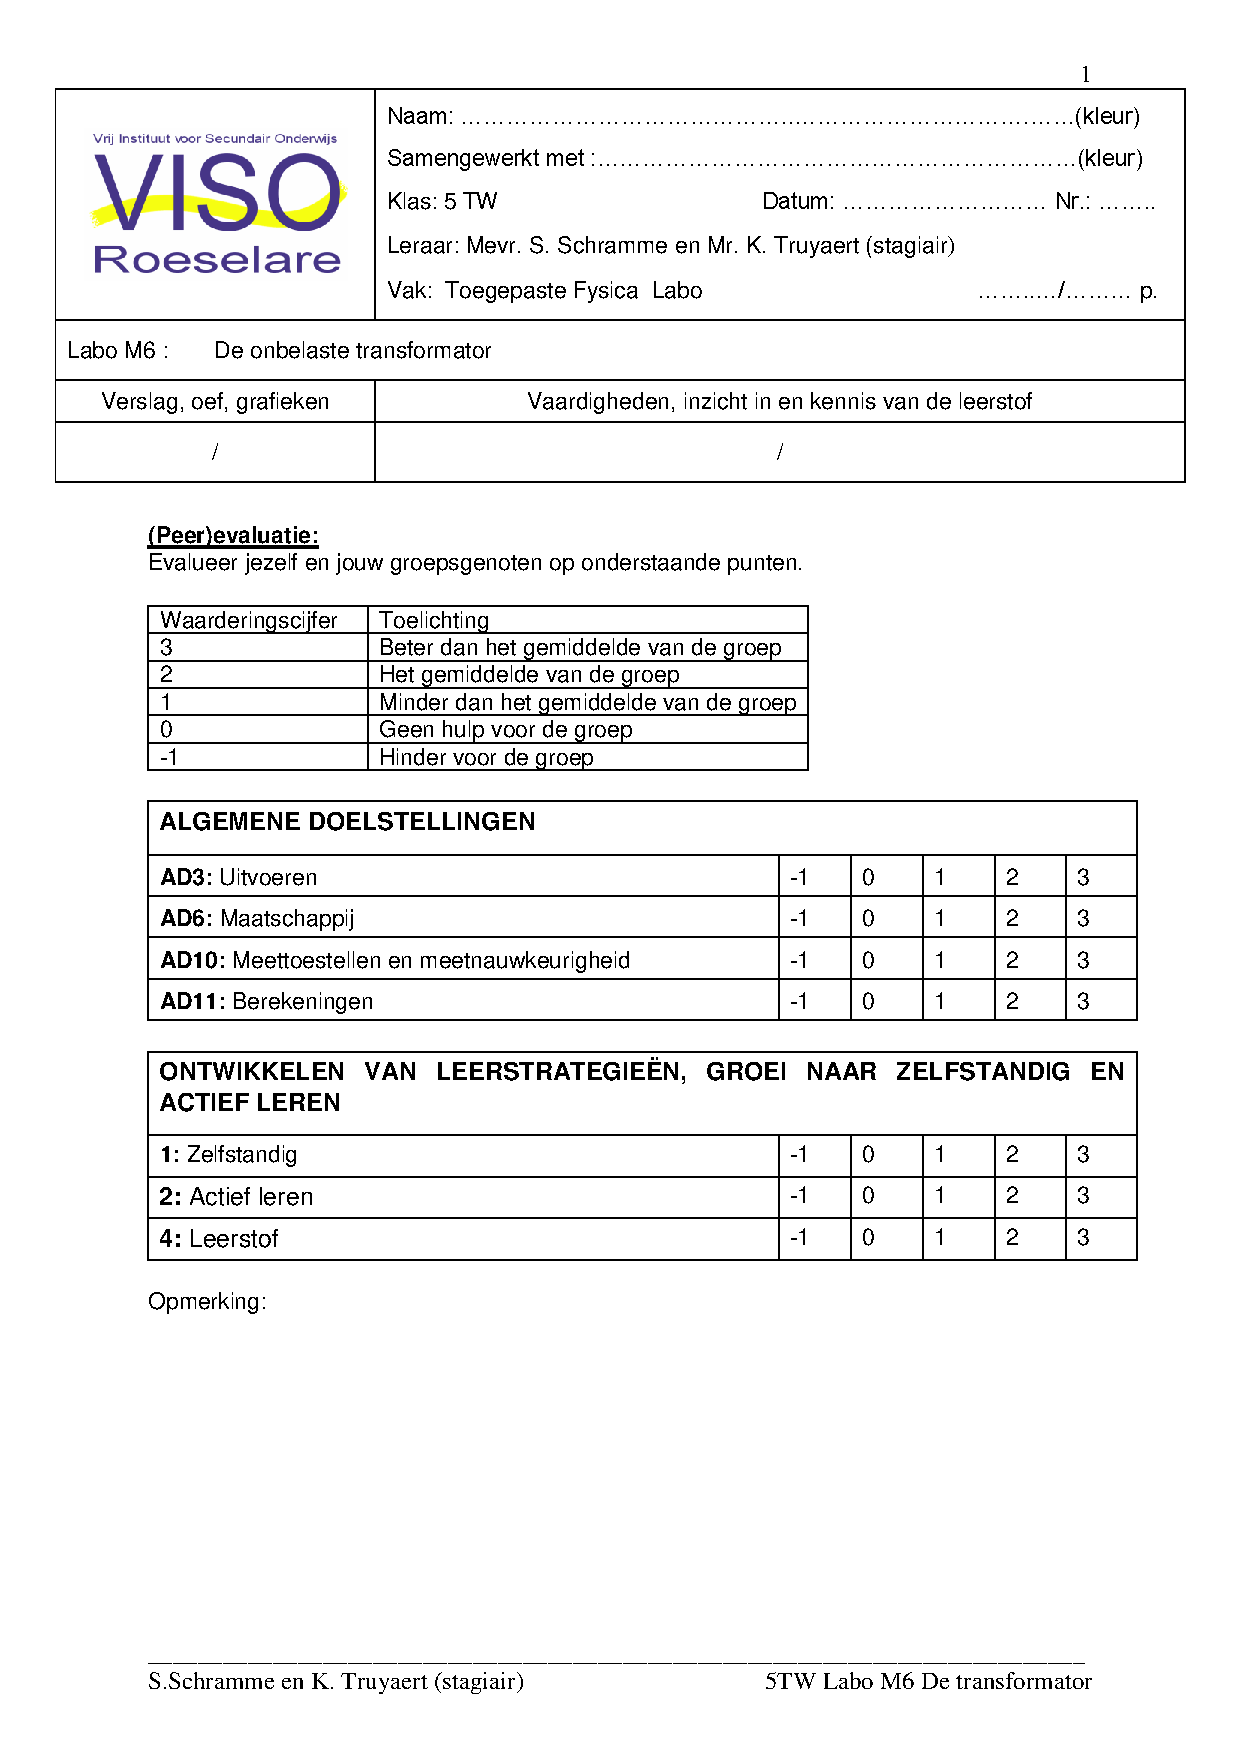
\includepdf[scale = 0.8,pages = 1,pagecommand=\subsubsection{Labo les 22-23}]{M6_DeTransformator1920}
\includepdf[scale = 0.8,pages =2-,pagecommand=]{M6_DeTransformator1920}







%\subsection*{Bijlage 5.1: slides introductie}

%
%\subsection*{Bijlage 1.2: bordschema theorie}
%\begin{center}
%	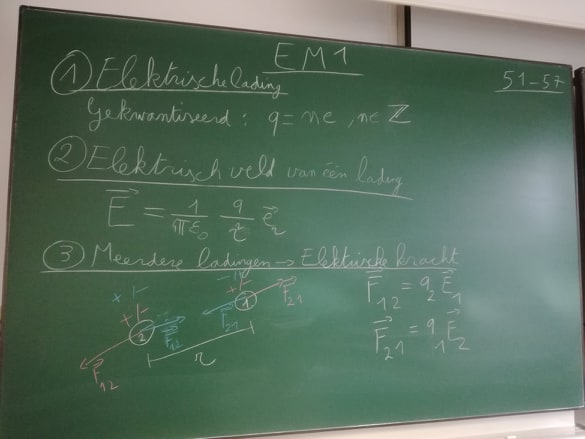
\includegraphics[width=0.9\textwidth]{Bord1a}
%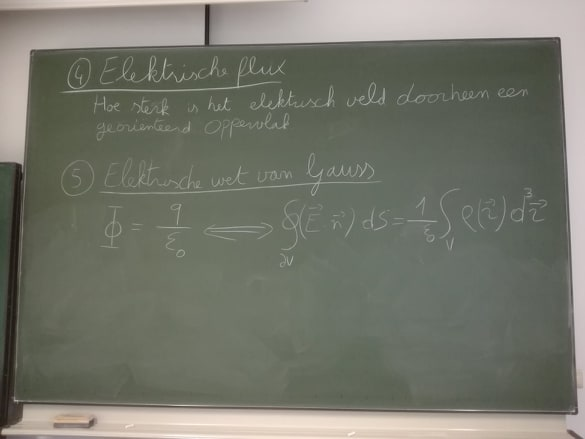
\includegraphics[width=0.9\textwidth]{Bord1b}
%\end{center}
%\newpage
%
%
%\includepdf[scale = 0.8,pages = 17,pagecommand=\subsection*{Bijlage 1.3: opgeloste oefeningen}]{Observaties_OpgelosteOef}
%\includepdf[scale = 0.8,pages =18-20,pagecommand=]{Observaties_OpgelosteOef}
%
%
%
%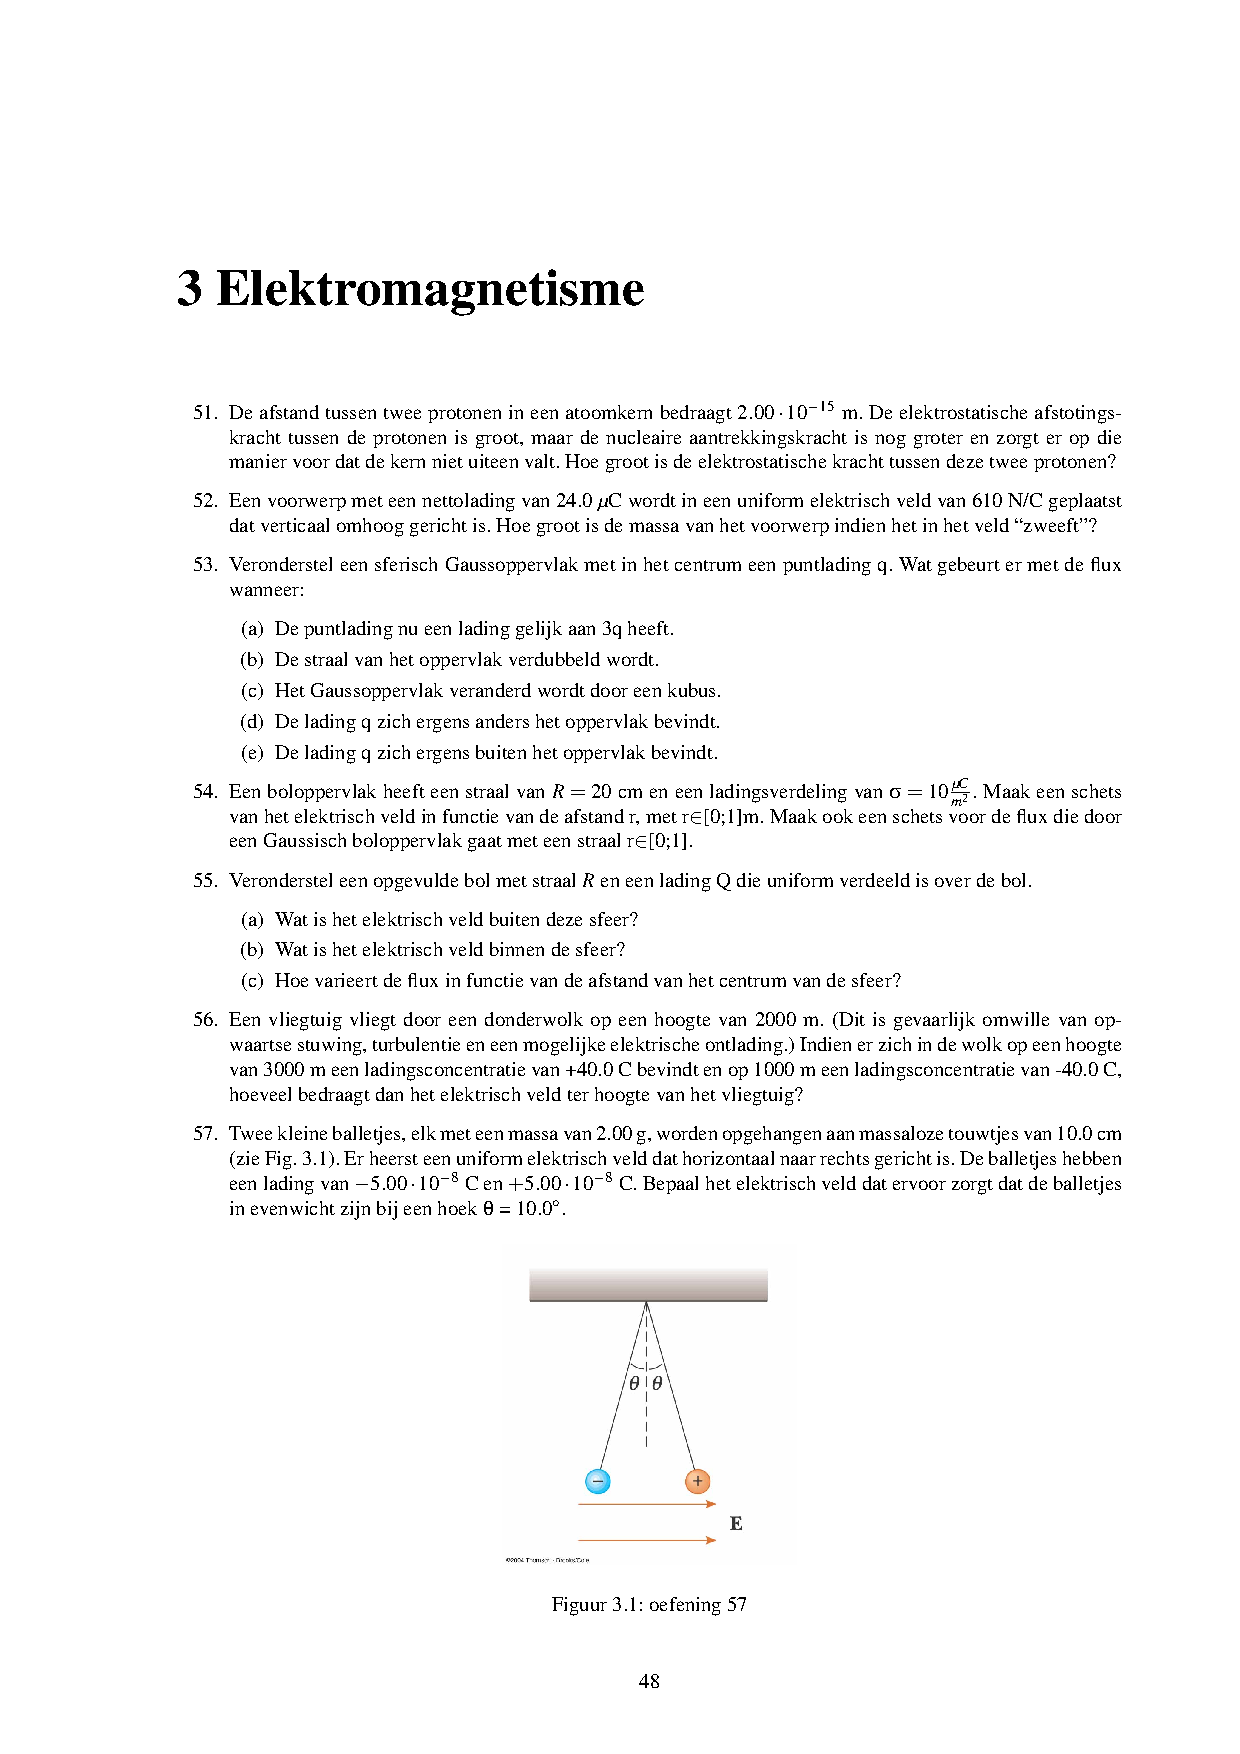
\includepdf[scale = 0.95,pages = 1,pagecommand=\subsection*{Bijlage 1.4: oefeningenbundel elektromagnetisme}]{OefeningenBundel}
%\includepdf[scale = 0.95,pages =2-,pagecommand=]{OefeningenBundel}